\section{Web-app amministratori}
\subsection{Introduzione}
La web app costituisce l'interfaccia tramite la quale l'amministratore può interagire col sistema.
Le funzionalità offerte sono:
\begin{itemize}
	\item login e logout;
	\item visualizzazione delle stanze e delle postazioni con i relativi stati;
	\item aggiunta, rimozione e modifica di stanze e postazioni;
	\item impostazione di postazioni come guaste;
	\item impostazione di stanze come inaccessibili;
	\item visualizzazione delle credenziali degli utenti;
	\item aggiunta, rimozione e modifica di credenziali;
	\item visualizzazione e scaricamento report sulle occupazioni e sulle igienizzazioni;
	\item visualizzazione di notifiche riguardanti il salvataggio dei dati sulla blockchain.
\end{itemize}

\subsection{Requisiti e installazione}
Il codice sorgente della web-app è pubblicato su GitHub all'indirizzo \url{https://github.com/DPCMGroup/bc19-webapp}.
Lo si può scaricare compresso in formato zip direttamente dal sito o, se si ha già installato il programma git, eseguendo il comando
\begin{verbatim}
	git clone https://github.com/DPCMGroup/bc19-webapp
\end{verbatim}

\subsubsection{Linguaggi}
\paragraph{Typescript}
Superset del linguaggio Javascript.

\paragraph{HTML}
Linguaggio di markup utilizzato per definire la struttura delle pagine web.

\paragraph{CSS}
Linguaggio per la definizione dello stile grafico delle pagine web.

\subsubsection{Tecnologie}
\paragraph{Node.js}
Programma focalizzato sull'esecuzione di codice javascript al di fuori del browser.
Per l'installazione fare riferimento alla pagina \url{https://nodejs.org/en/download/} 
\paragraph{npm}
Acronimo di Node Package Manager, permette di ottenere le librerie necessarie allo sviluppo.
Si ottiene insieme a Node.js tramite l'installazione di quest'ultimo.
\paragraph{Angular}
Framework per applicazioni web.
Per l'installazione fare riferimento alla pagina \url{https://angular.io/guide/setup-local#install-the-angular-cli}
\paragraph{Bootstrap}
Framework per la creazione di pagine web.
Per l'integrazione di bootstrap in angular fare riferimento alla pagina \url{https://www.npmjs.com/package/@ng-bootstrap/ng-bootstrap#installation}

\subsubsection{Test}

\subsection{IDE}
Per lo sviluppo abbiamo utilizzato l'IDE WebStorm. Per la sua installazione riferirsi alla pagina \url{https://www.jetbrains.com/webstorm/download/}

\subsection{Architettura}
L'architettura della web-app segue il modello a componenti imposto da Angular, che, a sua volta, si basa sul pattern Model-View-ViewModel, descritto dall'immagine sottostante.
\begin{figure}[H]
	\centering
	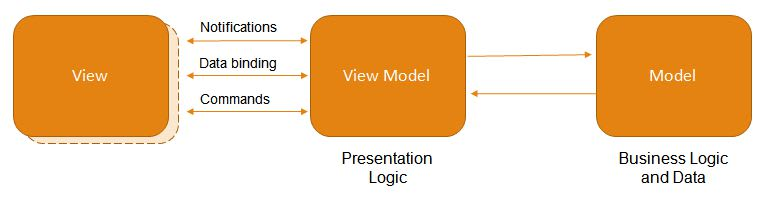
\includegraphics[width=15cm]{res/images/mvvm.jpg}
	\caption{Model-View-ViewModel}
	\label{fig:Model-View-ViewModel}
\end{figure}
Secondo questo modello la parte visiva del sito viene suddivisa in componenti, e ognuna di queste parti viene controllata da una diversa classe.
La parte visiva viene chiamata view, mentre la parte di controllo viene chiamata view model.
Un componente è costituito da 4 file. Nel seguente esempio è rappresentato un componente chiamato base.
\begin{verbatim}
	base.component.css
	base.component.html
	base.component.test.ts
	base.component.ts
\end{verbatim}
I file contengono, nell'ordine:
\begin{itemize}
	\item lo stile grafico del componente definito in css;
	\item la struttura del componente definito in html;
	\item i test definiti per il componente, scritti typescript;
	\item il codice che definisce la logica del componente, scritto in typescript;
\end{itemize}

\subsection{Diagrammi dei package}
\subsection{Diagrammi delle classi}
I diagrammi seguenti sono scritti secondo la sintassi UML2.0. Le descrizioni testuali degli attributi e dei metodi delle classi riprendono alcune notazioni del linguaggio UML:
\begin{itemize}
	\item +/*/- prima del nome di un attributo o metodo indica che esso è, rispettivamente, pubblico, protetto o privato;
	\item i metodi e gli attributi il cui nome è sottolineato (\underline{nome\_esempio}) sono statici.
\end{itemize}
\subsubsection{Login}
\subsubsection{Gestione stanze e postazioni}
\begin{figure}[H]
	\centering
	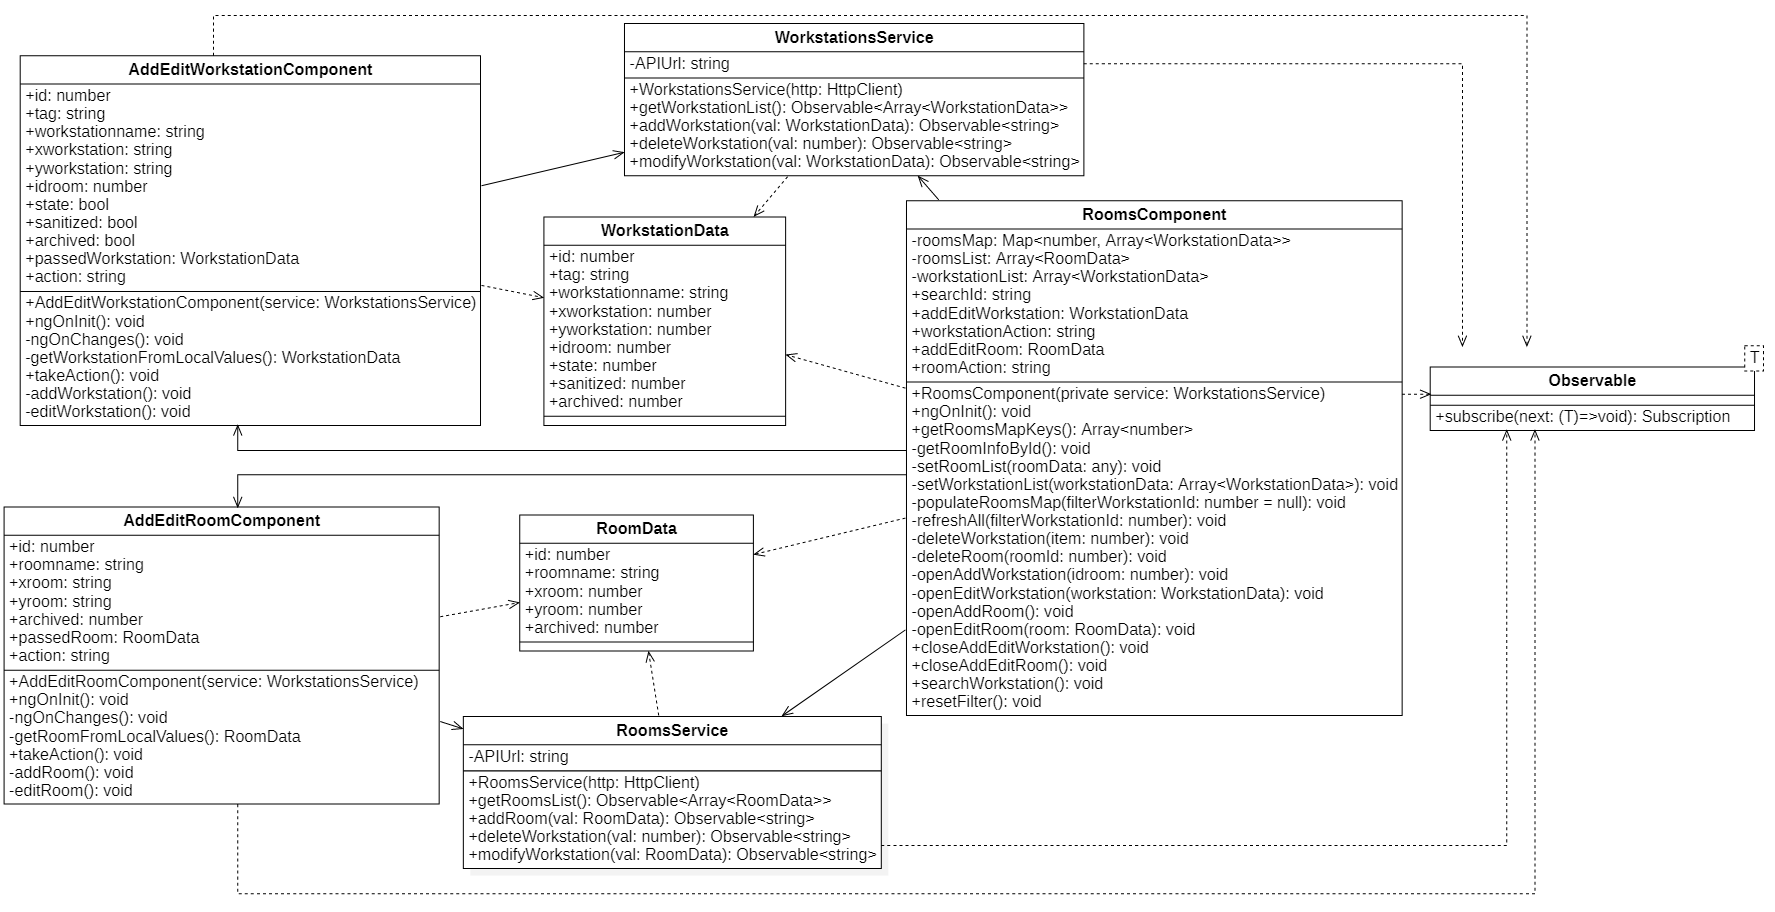
\includegraphics[width=18cm]{res/images/webapp-visualAddEditStanzePostazioni-diagrammaClassi.png}
	\caption{Diagramma delle classi per la gestione delle stanze e delle postazioni}
	\label{fig:DiagrammaClassiStanzePostazioni}
\end{figure}

\paragraph{Classi}
\subparagraph{RoomsComponent}
\textbf{Attributi}
\begin{itemize}
	\item \texttt{- roomMap: Map<number, Array<WorkstationData>>} \\
		È una Map in cui ad ogni stanza sono assegnate le sue postazione, ovvero quelle con \texttt{idroom} uguale all'\texttt{id} della stanza.
	\item \texttt{- roomsList: Array<RoomsData>} 
	\item \texttt{- workstationList: Array<Workstation>} 
	\item \texttt{+ searchId: string} 
	\item \texttt{+ addEditWorkstation: WorkstationData} 
	\item \texttt{+ workstationAction: string} 
	\item \texttt{+ addEditRoom: RoomData} 
	\item \texttt{+ roomAction: string} 
\end{itemize}
\textbf{Metodi}
\begin{itemize}
	\item \texttt{+ constructor(- service: SharedService, - cd: ChangeDetectorRef)} 
	\item \texttt{+ ngOnInit(): void} 
	\item \texttt{+ getRoomsMapKeys(): Array<number>} 
	\item \texttt{- getRoomInfoById(): void} 
	\item \texttt{- setRoomList(roomData: any): void} 
	\item \texttt{- setWorkstationList(workstationData: Array<WorkstationData>): void} 
	\item \texttt{- populateRoomsMap(filterWorkstationId: number): void} 
	\item \texttt{- refreshAll(filterWorkstationid: number): void} 
	\item \texttt{- deleteWorkstation(item: number): void} 
	\item \texttt{- deleteRoom(roomId: number): void} 
	\item \texttt{- openAddWorkstation(idroom: number): void} 
	\item \texttt{- openEditWorkstation(workstation: WorkstationData): void} 
	\item \texttt{- openAddRoom(): void} 
	\item \texttt{- openEditRoom(room: RoomData): void} 
	\item \texttt{+ closeAddEditWorkstation(): void} 
	\item \texttt{+ closeAddEditRoom(): void} 
	\item \texttt{+ searchWorkstation(): void} 
	\item \texttt{+ resetFilter(): void} 
\end{itemize}
	
\subparagraph{AddEditWorkstationComponent}
\textbf{Attributi}
\begin{itemize}
	\item \texttt{+ id: number } 
	\item \texttt{+ tag: string } 
	\item \texttt{+ workstationname: string } 
	\item \texttt{+ xworkstation: string } 
	\item \texttt{+ yworkstation: string } 
	\item \texttt{+ idroom: number } 
	\item \texttt{+ state: bool } 
	\item \texttt{+ sanitized: bool } 
	\item \texttt{+ archived: bool } 
	\item \texttt{+ passedWorkstation: WorkstationData } 
	\item \texttt{+ action: string} 
\end{itemize}
\textbf{Metodi}
\begin{itemize}
	\item \texttt{+ AddEditWorkstationComponent(service: WorkstationsService) }
	\item \texttt{+ ngOnInit(): void }
	\item \texttt{- ngOnChanges(): void }
	\item \texttt{- getWorkstationFromLocalValues(): WorkstationData }
	\item \texttt{+ takeAction(): void }
	\item \texttt{- addWorkstation(): void }
	\item \texttt{- editWorkstation(): void}
\end{itemize}
\subparagraph{AddEditRoomComponent}
\textbf{Attributi}
\begin{itemize}
	\item \texttt{+ id: number 	}
	\item \texttt{+ roomname: string 	}
	\item \texttt{+ xroom: string 	}
	\item \texttt{+ yroom: string 	}
	\item \texttt{+ archived: number 	}
	\item \texttt{+ noticeChangeVariable: boolean 	}
	\item \texttt{+ passedRoom: RoomData 	}
	\item \texttt{+ action: string}
\end{itemize}
\textbf{Metodi}
\begin{itemize}
	\item \texttt{+ AddEditRoomComponent(service: WorkstationsService) 	}
	\item \texttt{+ ngOnInit(): void 	}
	\item \texttt{- ngOnChanges(): void 	}
	\item \texttt{- getRoomFromLocalValues(): RoomData 	}
	\item \texttt{+ takeAction(): void 	}
	\item \texttt{- addRoom(): void 	}
	\item \texttt{- editRoom(): void}
\end{itemize}
\subparagraph{WorkstationsService}
\textbf{Attributi}
\begin{itemize}
	\item \texttt{- APIUrl: string}
\end{itemize}
\textbf{Metodi}
\begin{itemize}
	\item \texttt{+ WorkstationsService(http: HttpClient) 	}
	\item \texttt{+ getWorkstationList(): Observable<Array<WorkstationData>> 	}
	\item \texttt{+ addWorkstation(val: WorkstationData): Observable<string> 	}
	\item \texttt{+ deleteWorkstation(val: number): Observable<string> 	}
	\item \texttt{+ modifyWorkstation(val: WorkstationData): Observable<string>}
\end{itemize}
\subparagraph{RoomsService}
\textbf{Attributi}
\begin{itemize}
	\item \texttt{- APIUrl: string}
\end{itemize}
\textbf{Metodi}
\begin{itemize}
	\item \texttt{+ RoomsService(http: HttpClient) 	}
	\item \texttt{+ getRoomsList(): Observable<Array<RoomData>> 	}
	\item \texttt{+ addRoom(val: RoomData): Observable<string> 	}
	\item \texttt{+ deleteWorkstation(val: number): Observable<string> 	}
	\item \texttt{+ modifyWorkstation(val: RoomData): Observable<string>}
\end{itemize}
\subparagraph{WorkstationData}
\textbf{Attributi}
\begin{itemize}
	\item \texttt{+ id: number 	}
	\item \texttt{+ tag: string 	}
	\item \texttt{+ workstationname: string 	}
	\item \texttt{+ xworkstation: number 	}
	\item \texttt{+ yworkstation: number 	}
	\item \texttt{+ idroom: number 	}
	\item \texttt{+ state: number 	}
	\item \texttt{+ sanitized: number 	}
	\item \texttt{+ archived: number}
\end{itemize}
\subparagraph{RoomData}
\textbf{Attributi}
\begin{itemize}
	\item \texttt{+ id: number 	}
	\item \texttt{+ roomname: string 	}
	\item \texttt{+ xroom: number 	}
	\item \texttt{+ yroom: number 	}
	\item \texttt{+ archived: number}
\end{itemize}
\subparagraph{Observable<T>}
\textbf{Metodi}
\begin{itemize}
	\item \texttt{+ subscribe(next: (T)=>void): Subscription}
\end{itemize}

\subsubsection{Gestione credenziali}
\subsubsection{Sezione report}
\subsubsection{Sezione notifiche}
\subsection{Diagrammi di sequenza}
\subsubsection{Login}
\subsubsection{Gestione stanze e postazioni}
\begin{figure}[H]
	\centering
	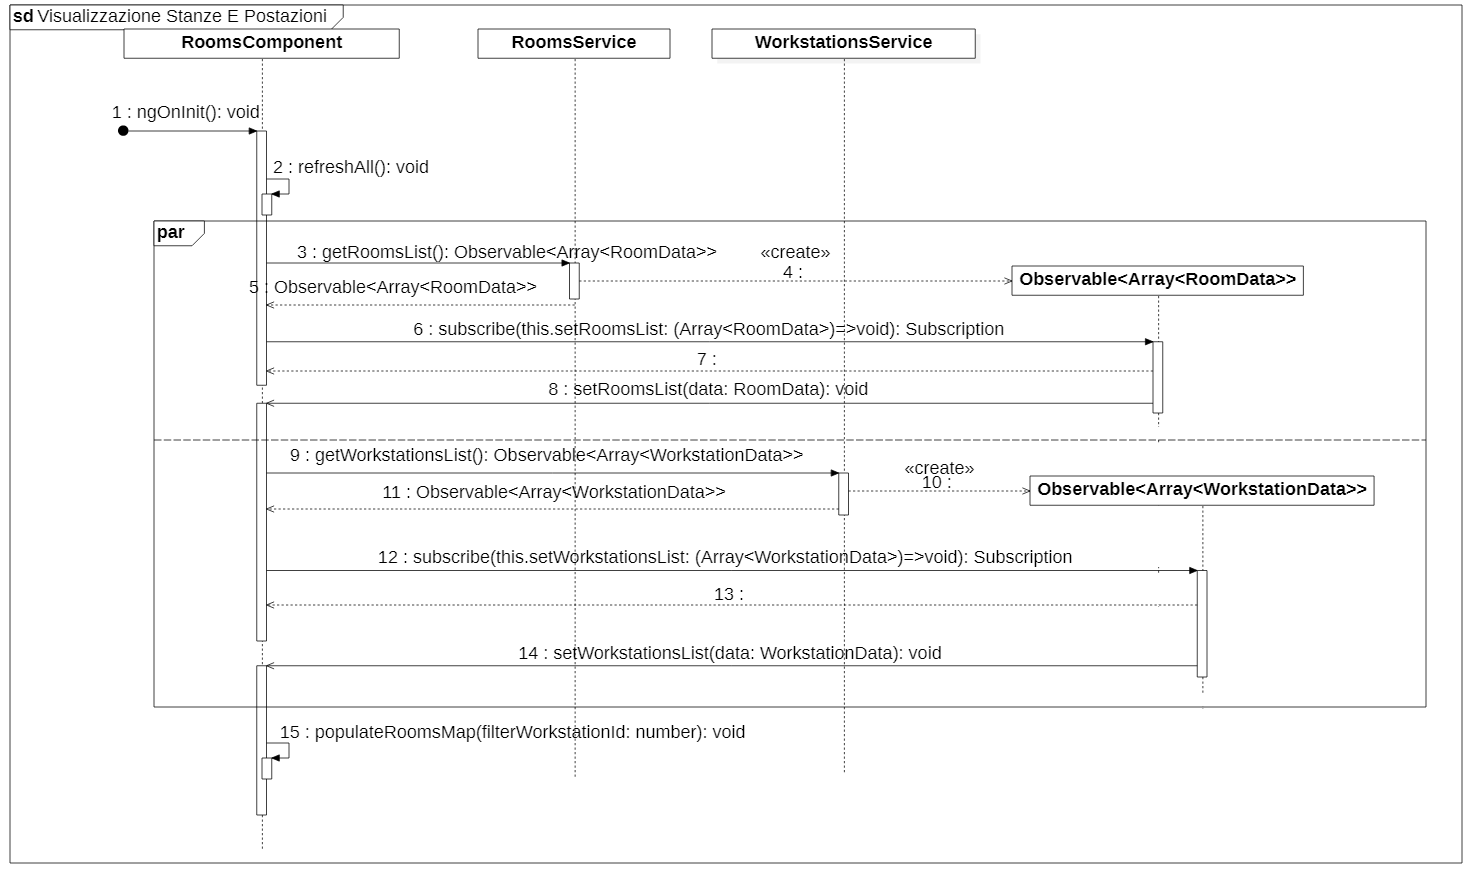
\includegraphics[width=18cm]{res/images/webapp-visualStanzePostazioni-diagrammaSequenza.png}
	\caption{Diagramma di sequenza per la visualizzazione delle stanze e delle postazioni}
	\label{fig:DiagrammaSequenzaStanzePostazioni1}
\end{figure}
\begin{figure}[H]
	\centering
	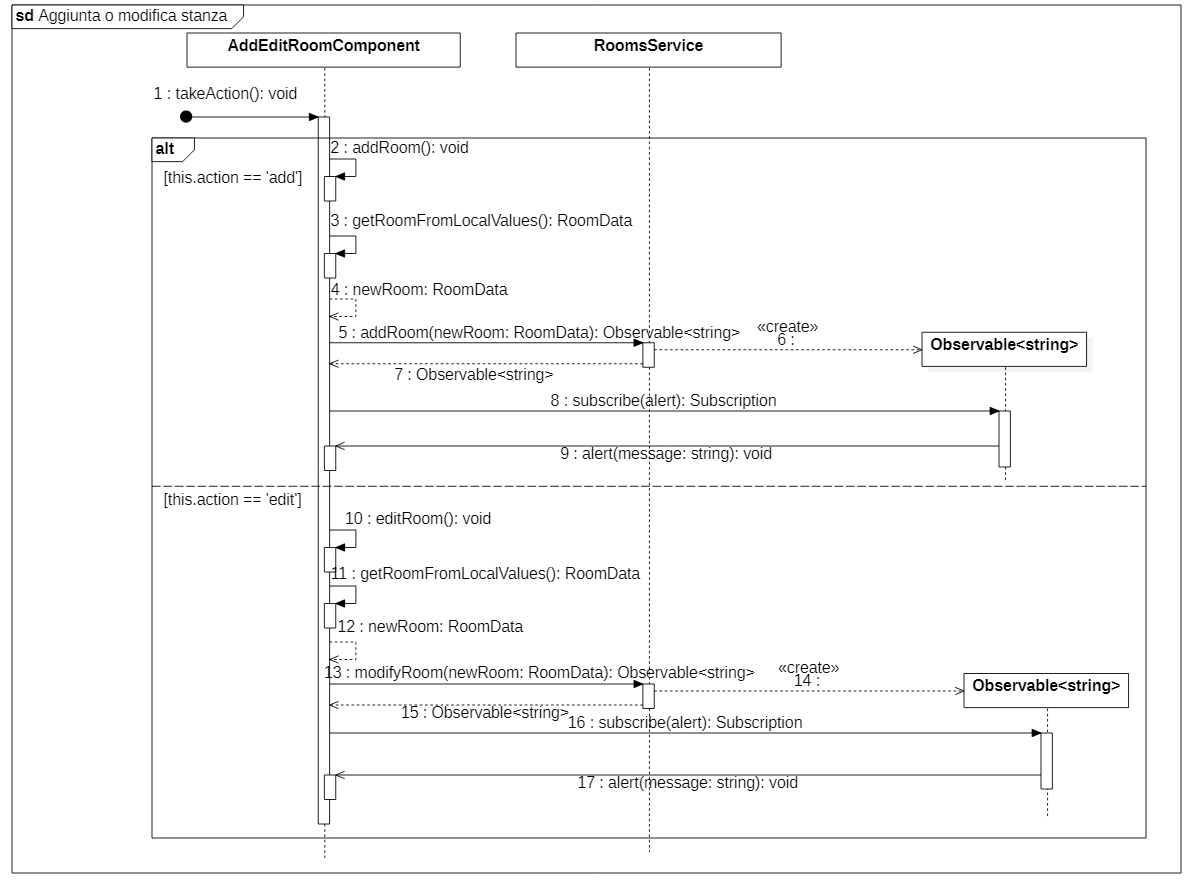
\includegraphics[width=18cm]{res/images/webapp-addEditStanzePostazioni-diagrammaSequenza.png}
	\caption{Diagramma di sequenza per l'aggiunta e la modifica di una stanza}
	\label{fig:DiagrammaSequenzaStanzePostazioni2}
\end{figure}
\subsubsection{Gestione credenziali}
\subsubsection{Sezione report}
\subsubsection{Sezione notifiche}



